\section{习题参考答案}
\subsection*{计算题}
\begin{enumerate}
    \item 如图所示 \ref{Fig:56}, 有一长$l$的带电细杆.
    \begin{enumerate}
        \item[(1)] 电荷均匀分布, 线密度为$+\lambda$, 则杆上距原点$x$处的线元$\mathrm{d}x$对$P$点的点电荷$q_0$的电场力为何? $q_0$受的总电场力为何?
        \item[(2)] 若$\lambda=\varepsilon_0 l$(正电荷), $a=4l$, 则$P$点的电场强度是多少? (如图所示选择坐标系).
    \end{enumerate}
    \begin{figure}[H]
        \centering
        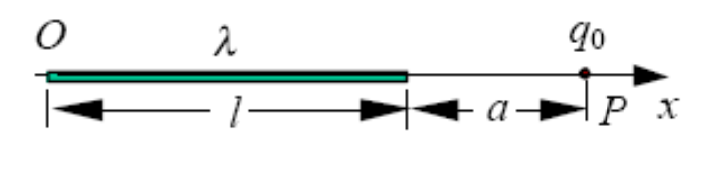
\includegraphics[width=0.15\textheight]{fig56}
        \caption{如图.}\label{Fig:56}
    \end{figure}
    \begin{solution}
        如图:
        \begin{figure}[H]
            \centering
            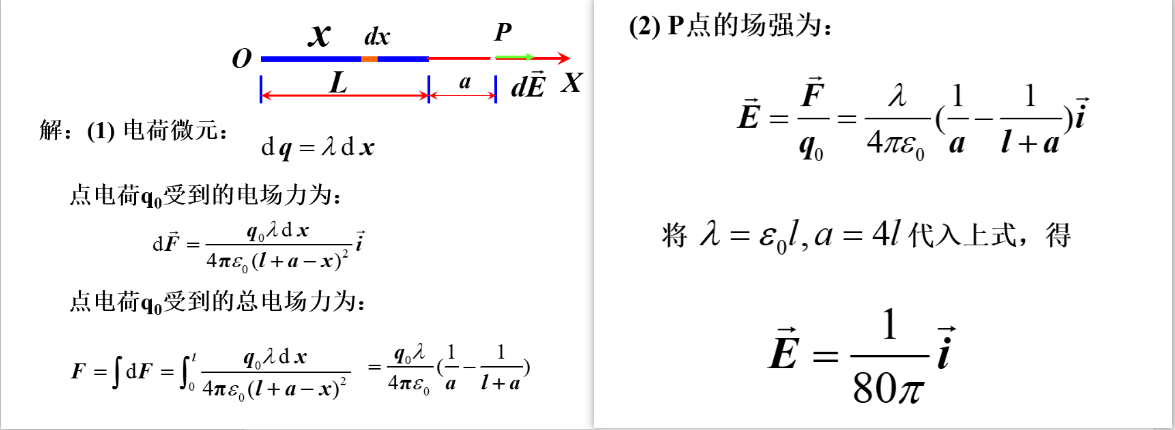
\includegraphics[width=0.55\textheight]{ans35}
        \end{figure}
    \end{solution}
    \item 一半径为$R$的“无限长”圆柱形带电体, 其电荷体密度为$\rho=Ar(r<R)$, 式中$A$为常数, 试求:
    \begin{enumerate}
        \item[(1)] 圆柱体内, 外各点场强大小分布;
        \item[(2)] 选距离轴线的距离为$R_0(R_0>R)$处为电势零点, 计算圆柱体内, 外各点的电势分布.
    \end{enumerate}
    \begin{solution}
        如图:
        \begin{figure}[H]
            \centering
            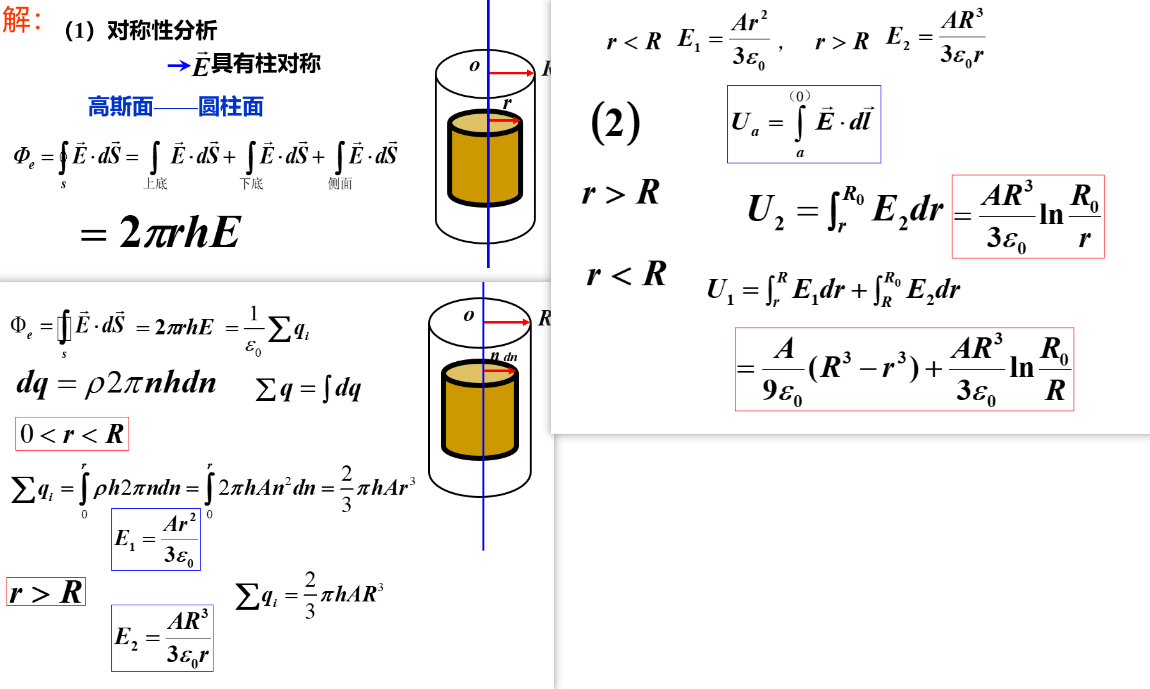
\includegraphics[width=0.55\textheight]{ans36}
        \end{figure}
    \end{solution}
    \item 如图\ref{Fig:57},半径为$R$的圆弧形细塑料棒, 两端空隙对中心张角为$2\theta_0$, 线电荷密度为$\lambda$的正电荷均匀地分布在棒上. 求:
    \begin{enumerate}
        \item[(1)] 用连续带电体场强叠加原理计算圆心$O$处场强的大小和方向.
        \item[(2)] 圆心处的电势.
    \end{enumerate}
    \begin{figure}[H]
        \centering
        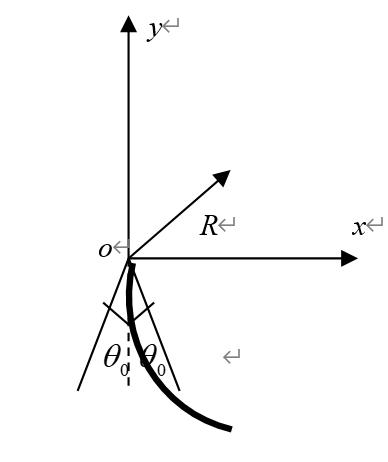
\includegraphics[width=0.15\textheight]{fig57}
        \caption{如图.}\label{Fig:57}
    \end{figure}
     \begin{solution}
        如图:
        \begin{figure}[H]
            \centering
            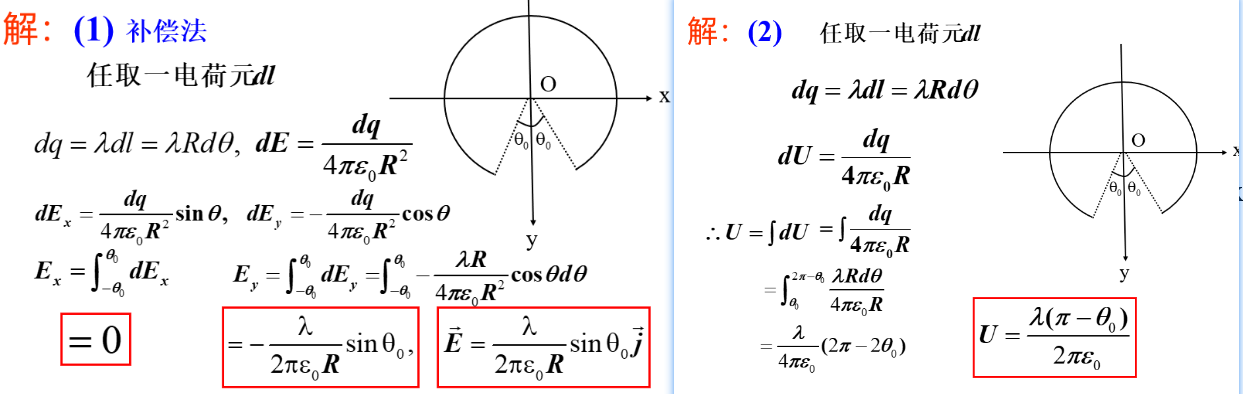
\includegraphics[width=0.55\textheight]{ans37}
        \end{figure}
    \end{solution}
    \item  一环形薄片由细绳悬吊着, 环的外半径为$R$, 内半径为$R/2$, 并有电荷$Q$均匀分布在环面上. 细绳长$3R$, 也有电荷$Q$均匀分布在绳上, 如图所示\ref{Fig:58}. 试求圆环中心$O$处的电场强度(圆环中心$O$在细绳延长线上)
    \begin{figure}[H]
        \centering
        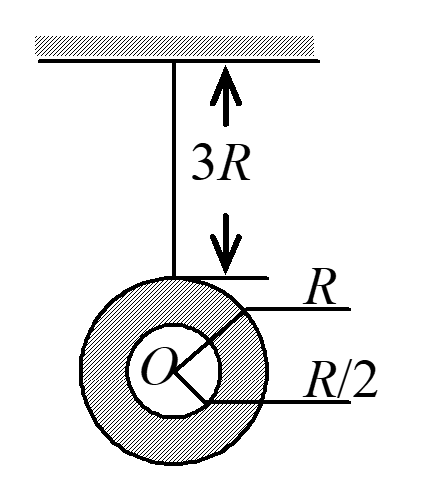
\includegraphics[width=0.15\textheight]{fig58}
        \caption{如图.}\label{Fig:58}
    \end{figure}
    \begin{solution}
        如图:
        \begin{figure}[H]
            \centering
            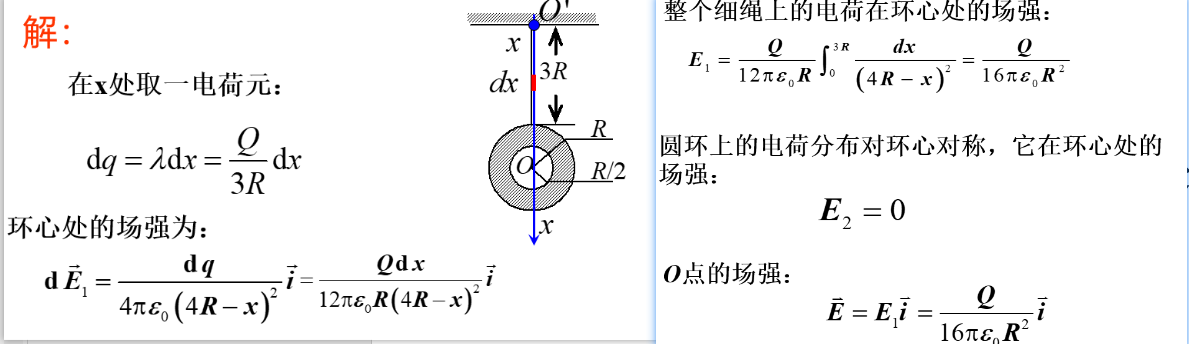
\includegraphics[width=0.55\textheight]{ans38}
        \end{figure}
    \end{solution}
\end{enumerate}